
\documentclass{article}

\usepackage[latin1]{inputenc}
\usepackage{tikz}

\usepackage{pgfplots}

% GNUPLOT required
\begin{document}
\pagestyle{empty}


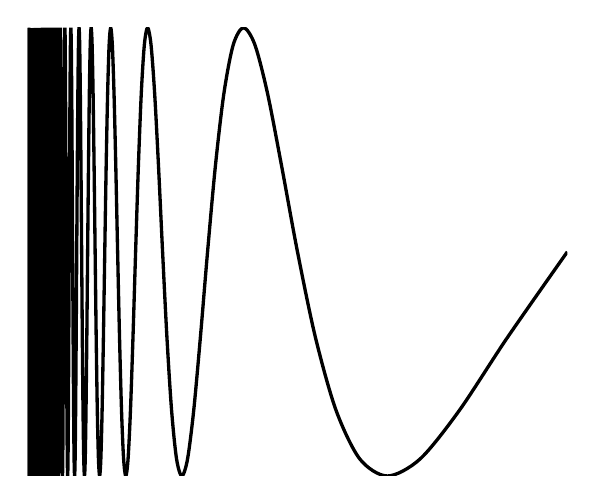
\begin{tikzpicture}
        \begin{axis}[
            domain=0:2, xmin=0, xmax=1, ymin=-1, ymax=1,
            xlabel=$x$, ylabel=$y$,
            %every axis y label/.style={at=(current axis.above origin),anchor=south},
            %every axis x label/.style={at=(current axis.right of origin),anchor=west},
            hide axis,
          ]
          %\addplot [very thick,black, smooth,domain=(0.01:6)] {sin(1/x)};
          %\addplot [domain=0.1:2,smooth,samples=100] {sin(deg((pi/(x)))}; 
          \addplot [domain=1:501,smooth,very thick,samples=4000]({1/(x)},{sin(deg(pi*x))}); 
          \addplot [domain=-1:1,line width=20pt,samples=4]({0},{(x)}); 

          \end{axis}
\end{tikzpicture}


\end{document}
